\newpage
\section{CPU reduction}
\begin{figure}[h]
    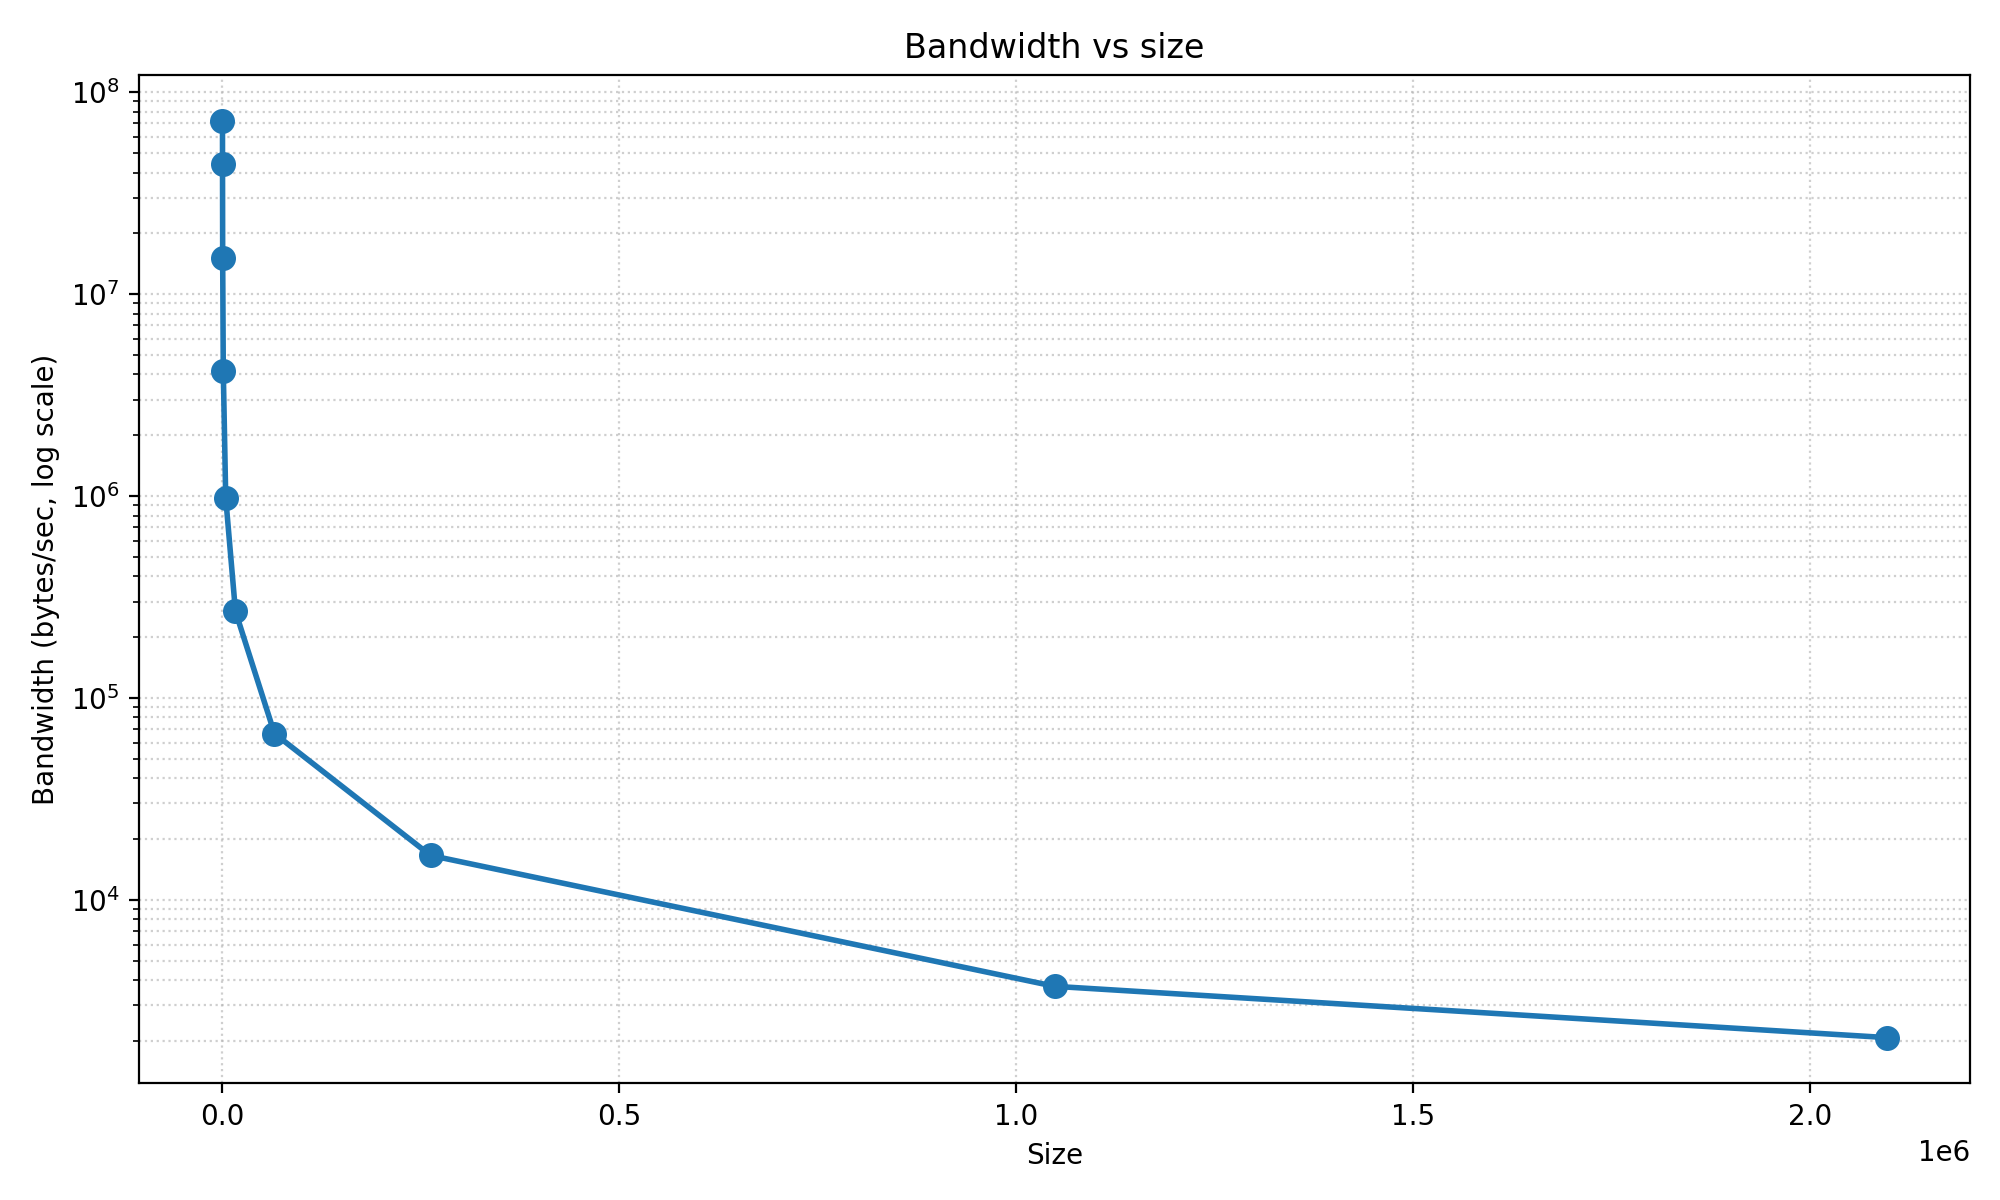
\includegraphics[width=1.0\textwidth]{../noah/plots/6_2/bandwidth_vs_size.png}
    \caption{CPU: Bandwith vs. size of data}
    \label{fig:2}
\end{figure}
\ref{fig:2} shows the bandwith of the kernel of the naive CPU implementation. Measurements are a done with an average over 10 runs.\\
What can be observed is that the bandwith decreases with increasing data sizes. This is due to the fact that, with data getting larger, higher and thus slower levels of the cache hierarchy need to bu used.